% Mention the two models, and describe the architecture

% the two models:

%     TF-IDF + Logistic Regression
%     TF-IDF + LinearSVM

% The hyperparameter search for TF-IDF + Logistic Regression

%     C: [0.01, 0.1, 1.0, 100.0]

% The hyperparameter search for TF-IDF + LinearSVM

%     C: [0.01, 0.1, 1.0, 10.0, 100.0]
%     loss: ["hinge", "squared_hinge"]

% Mention what was the best hyperparameters, and what was the dev accuracy, for each model

In this section, we describe the two models we implemented for the text classification task: TF-IDF + Logistic Regression and TF-IDF + LinearSVM. Both models utilize Term Frequency-Inverse Document Frequency (TF-IDF) for feature extraction, which transforms the textual data into a numerical representation based on the importance of words in the documents.

The model architecture is shown in Figure \ref{fig:model_architecture}. The input text is first preprocessed and then transformed into TF-IDF features. These features are then fed into either a Logistic Regression classifier or a Linear Support Vector Machine (SVM) for classification.

\begin{figure}[ht]
    \centering
    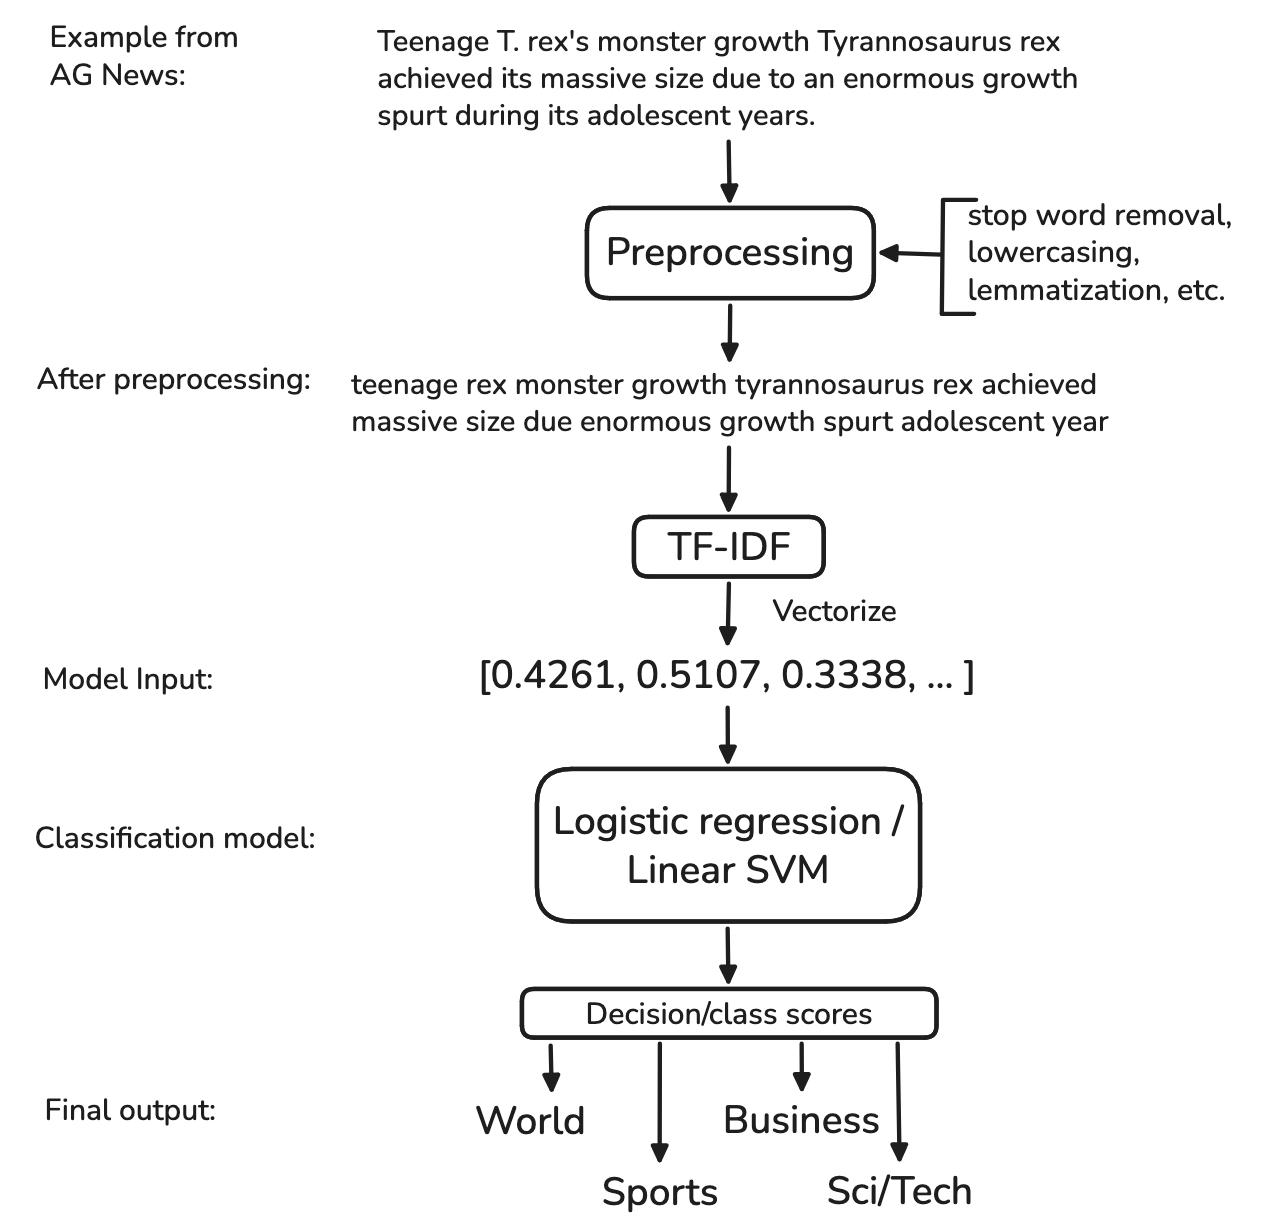
\includegraphics[width=0.6\textwidth]{../figures/model_architecture.png}
    \caption{Model architecture for TF-IDF + Logistic Regression and TF-IDF + LinearSVM. The figure shows a random sample from the training set, which is preprocessed and transformed into TF-IDF features before being fed into the classifiers.}
    \label{fig:model_architecture}
\end{figure}

For the TF-IDF + Logistic Regression model, we performed a hyperparameter search over the regularization strength parameter \( C \) with the values [0.01, 0.1, 1.0, 100.0]. The best hyperparameters for this model were found to be \( C = XXX \), which yielded a development accuracy of approximately XXX\%.

For the TF-IDF + LinearSVM model, we conducted a more extensive hyperparameter search over both the regularization strength \( C \) and the loss function. The values for \( C \) were [0.01, 0.1, 1.0, 10.0, 100.0], and the loss functions considered were "hinge" and "squared\_hinge". The best hyperparameters for this model were \( C = XXX \) and loss function = "XXX", resulting in a development accuracy of approximately XXX\%.
